\documentclass[11pt,a4paper]{article}

\usepackage{main}
\usepackage{cours}

\renewcommand{\typedocument}{Cours}
\renewcommand{\classe}{3e}
\renewcommand{\titre}{Signaux}

\begin{document}

\pagination

\creertitre{Signaux sonores et lumineux}

Nous percevons le monde grâce à des \important{signaux}. La \important{lumière} nous permet de voir, le \important{son} nous permet d'entendre : ce sont deux signaux qui transportent une information.

\partie{La lumière}

\souspartie{Sources primaires et objets diffusants}

Il existe deux types de sources de lumière.

Une \important{source primaire} est un objet qui produit sa propre lumière.

\exemple{le Soleil, une bougie, l'écran d'un téléphone.}

Un \important{objet diffusant} renvoie dans toutes les directions une partie de la lumière qu'il reçoit. On ne peut le voir que s'il est éclairé.

\exemple{la Lune (éclairée par le Soleil), un écran de cinéma.}

\souspartie{Propagation et rayon lumineux}

La lumière se déplace en ligne droite dans un milieu homogène et \important{transparent} (comme le vide, l’air ou l’eau) : on parle de \important{propagation rectiligne} de la lumière.

On représente son trajet par un \important{rayon lumineux} : un segment fléché.

\partie{Le son}

\souspartie{Sources sonores et propagation du son}

Le son est produit par la \important{vibration} de la matière.

\exemple{Une corde de guitare, nos cordes vocales.}

Il ne peut se propager que dans un \important{milieu matériel} (solide, liquide ou gazeux). Il ne peut pas se propager dans le vide.

\souspartie{Fréquence, son grave et son aigu}

La \important{fréquence} d’un son correspond au nombre de vibrations par seconde et s’exprime en \important{Hertz (Hz)}.

Un son grave correspond à une basse fréquence et un son aigu correspond à une haute fréquence.

L’oreille humaine n’entend pas toutes les fréquences : le \important{domaine audible s'étend d'environ \SI{20}{Hz} à \SI{20000}{Hz}.} En dessous se trouvent les infrasons et au dessus les ultrasons.

\vspace*{-1em}

\begin{center}
    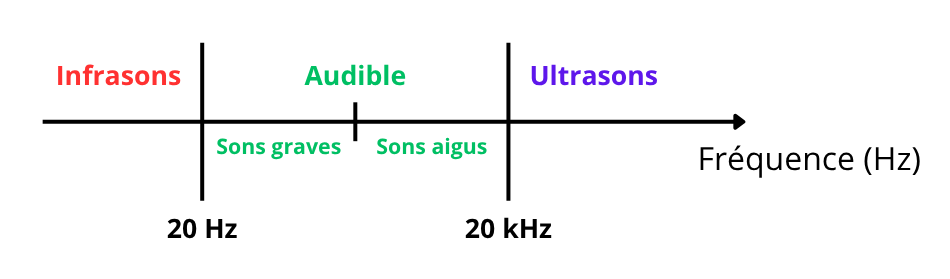
\includegraphics[width=0.6\textwidth]{images/frequences.png}
\end{center}

\vspace*{-1.5em}

\souspartie{Intensité sonore et risques}

L'\important{intensité sonore} (le « volume ») se mesure en \important{décibels (dB)} : plus un son est fort, plus le niveau en décibels est élevé. Un son trop intense, ou une exposition trop longue à un son fort, peut abîmer l'oreille.

\newpage

\partie{Ordres de grandeur et exemples}

La vitesse du son vaut :
\begin{itemize}
    \item \SI{340}{m/s} dans l'air,
    \item \SI{1500}{m/s} dans l'eau,
    \item le son ne se propage pas dans le vide.
\end{itemize}

La vitesse de la lumière vaut $\SI{3,00e8}{m/s}$ dans le vide. 

\exemple{\textbf{Une année-lumière correspond à la distance parcourue par la lumière en une année. Calculer cette distance en km.}\\
$t = 1 \text{ an} = 365 \times 24 \times 3600 \text{ s} = 3,1536 \times 10^7 \text{ s}$\\
$v = \SI{3,00e8}{m/s}$\\
$d = v \times t = 3,00 \times 10^{8} \times 3,1536 \times 10^7 = \SI{9,46e15}{m} = \SI{9,46e12}{km}$\\
Une année-lumière correspond à environ \SI{9,46e12}{km}.}

\exemple{\textbf{On entend un coup de tonnerre 3s après avoir vu l’éclair. A quelle distance est tombée la foudre ?}\\
On peut supposer que la lumière est instantanée, et donc le son a parcouru la distance entre la foudre et nous en 3s.\\
$v = \SI{340}{m/s}$\\
$t = 3 \text{ s}$\\
$d = v \times t = 340 \times 3 = \SI{1020}{m}$\\
La foudre est tombée à environ \SI{1,02}{km}.}

\end{document}